%Template
% !TeX spellcheck = de 
\documentclass[a4paper]{scrartcl}
\usepackage[utf8]{inputenc}
%\usepackage[ngerman]{babel}
\usepackage{geometry,forloop,fancyhdr,fancybox,lastpage}
\usepackage{listings}
\lstset{frame=tb,
	language=Java,
	aboveskip=3mm,
	belowskip=3mm,
	showstringspaces=false,
	columns=flexible,
	basicstyle={\small\ttfamily},
	numbers=left,
	numberstyle=\tiny\color{gray},
	keywordstyle=\color{blue},
	commentstyle=\color{dkgreen},
	stringstyle=\color{mauve},
	breaklines=true,
	breakatwhitespace=true,
	tabsize=3
}
\geometry{a4paper,left=3cm, right=3cm, top=3cm, bottom=3cm}
% Diese Daten müssen pro Blatt angepasst werden:
\newcommand{\NUMBER}{6}
\newcommand{\EXERCISES}{3}
% Diese Daten müssen einmalig pro Vorlesung angepasst werden:
\newcommand{\COURSE}{Einführung in Maschinelles Lernen}
\newcommand{\TUTOR}{TBD}
\newcommand{\STUDENTA}{Maria Heitmeier}
\newcommand{\STUDENTB}{Gwent Krause}
\newcommand{\STUDENTC}{Stefan Wezel}
\newcommand{\DEADLINE}{07.06.2018}




%Math
\usepackage{amsmath,amssymb,tabularx}

%Figures
\usepackage{graphicx,tikz,color,float}
\graphicspath{ {home/stefan/picures/} }
\usetikzlibrary{shapes,trees}

%Algorithms
\usepackage[ruled,linesnumbered]{algorithm2e}

%Kopf- und Fußzeile
\pagestyle {fancy}
\fancyhead[L]{\COURSE}
\fancyhead[C]{\STUDENTA, \STUDENTB, \STUDENTC\\}
\fancyhead[R]{\today}

\fancyfoot[L]{}
\fancyfoot[C]{}
\fancyfoot[R]{Seite \thepage}

%Formatierung der Überschrift, hier nichts ändern
\def\header#1#2{
	\begin{center}
		{\Large\bf Übungsblatt #1}\\
		{(Abgabetermin #2)}
	\end{center}
}

%Definition der Punktetabelle, hier nichts ändern
\newcounter{punktelistectr}
\newcounter{punkte}
\newcommand{\punkteliste}[2]{%
	\setcounter{punkte}{#2}%
	\addtocounter{punkte}{-#1}%
	\stepcounter{punkte}%<-- also punkte = m-n+1 = Anzahl Spalten[1]
	\begin{center}%
		\begin{tabularx}{\linewidth}[]{@{}*{\thepunkte}{>{\centering\arraybackslash} X|}@{}>{\centering\arraybackslash}X}
			\forloop{punktelistectr}{#1}{\value{punktelistectr} < #2 } %
			{%
				\thepunktelistectr &
			}
			#2 &  $\Sigma$ \\
			\hline
			\forloop{punktelistectr}{#1}{\value{punktelistectr} < #2 } %
			{%
				&	
			} &\\
			\forloop{punktelistectr}{#1}{\value{punktelistectr} < #2 } %
			{%
				&
			} &\\
		\end{tabularx}
	\end{center}
}

\begin{document}
\section*{Aufgabe 1}
\subsection*{(a)}
Das Ziel der PCA ist eine Repräsentation zu finden, die die Unterschiede in Daten möglichst gut darstellt. Dies geschieht indem eine Linearkombination gesucht wird, die (üblicherweise zwei) größten Varianzen der Daten enthält.\\
Klassenzugehörigkeit spielt bei der PCA üblicherweise keine Rolle. %TODO ned ganz sicher ob das stimmt



\subsection*{(b)}
Bei LDA versucht man wie bei PCA Linearkombinationen zu finden, die Daten gut repräsentiert. Allerdings möchte man hier noch Aussagen über Klassenzugehörigkeit treffen können. Wir benötigen also nicht zwingend die Linearkombination mit der größten Varianz, sonden die mit der größten Seperierbarkeit, also die die Daten in deutlich getrennte Cluster aufteilt.\\
Im Gegensatz zu PCA handelt es sich bei LDA um ein supervised learning Verfahren.



\subsection*{(c)}
$c-1$ Dimensionen.





\subsection*{(d)}
Bei der LDA wird versucht die Separation unterschiedlicher Klassen zu maximieren. Dies geschieht durch das maximieren des Verhältnisses von Abstand der Mittelwerte zu einer geraden und Streuung der Datenpunkte. Die Streuung können wir mithilfe der Scattermatrix berechnen.




\subsection*{(e)}
Die Streuung der Datenpunkte kann mithilfe der \text{within class scatter matrix} $S_W$ berechnet werden. Die Mittelwerte ergeben sich aus der \textit{between class scatter matrix} $S_B$.\\
Für die within class scatter matrix gilt:\\
$
S_W = S_1 + S_2
$\\
$S_1$ und $S_2$ ergeben sich aus:\\
$
S_i = \sum_{x\in\mathcal{D}_i}(x-m_i)\cdot(x-m_i)^T
$\\
\\
Für die between class scatter matrix gilt:\\
$
S_B = (m_1 - m_2)\cdot(m_1-m_2)^T
$\\
\\
Die Mat




\section*{Aufgabe 2}
\subsection*{a)}
z.z.: $$J_1(e) = \sum_{k=1}^{n} ||(m+(e|x_k - m)e) - x_k||^2$$
ist minimal für den Eigenvektor $e$ mit dem größten Eigenwert.\\
\underline{Beweis:}\\
Wir wählen für e den Einheitsvektor, für den gilt $||e|| = ee^T = 1$.
\begin{align*}
	J_1(e) &= \sum_{k=1}^{n} ||(m+(e|x_k - m)e) - x_k||^2\\
	&= \sum_{k=1}^{n} ||(m - x_k + e^T(x_k - m)e)||^2
\end{align*}
Für eine klarere Notation definieren wir im Folgenden $m-x_k = z_k$. Außerdem sei an dieser Stelle gesagt, dass nach der linearen Algebra gilt: Für zwei Vektoren $x,y \in \mathbb{R}^m$ gilt, dass $xy = yx$. Aber es gilt nicht: $xy^T = y^Tx$. Außerdem gilt: $(xy)^T = y^Tx^T$ und $(x + y)^T = x^T + y^T$. Mit diesen Regeln gilt nun:
\begin{align*}
	J_1(e) &= \sum_{k=1}^{n} ||z_k-e^Tz_ke||^2\\
	&=  \sum_{k=1}^{n} (z_k-e^Tz_ke)^T(z_k-e^Tz_ke)\\
	&= \sum_{k=1}^{n} z_k^Tz_k - z_k^Te^Tz_ke - (e^Tz_ke)^Tz_k + (e^Tz_ke)^T(e^Tz_ke)\\
	&= \sum_{k=1}^{n} z_k^Tz_k - (z_ke)^Tz_ke - (z_ke)^Tez_k + (z_ke)^Tee^T(z_ke)\\
	&= \sum_{k=1}^{n} z_k^Tz_k - (z_ke)^Tz_ke - (z_ke)^Tez_k + (z_ke)^T(z_ke)\\
	&= \sum_{k=1}^{n} z_k^Tz_k - (z_ke)^Tz_ke\\
	&= \sum_{k=1}^{n} z_k^Tz_k - e^Tz_k^Tz_ke\\
	&= \sum_{k=1}^{n} z_k^Tz_k - \sum_{k=1}^{n}e^Tz_k^Tz_ke\\
	&= \sum_{k=1}^{n} z_k^Tz_k - e^TSe\\
\end{align*}
Da $\sum_{k=1}^{n} z_k^Tz_k$ konstant ist, wird dieser Wert minimal, wenn $ e^TSe$ maximal ist. Das passiert genau dann, wenn $e$ der Eigenvektor des größten Eigenwerts von $S$ ist. \\
Dass wir $e$ als Einheitsvektor gewählt haben, spielt hier keine Rolle, da alle Vektoren mit $\frac{\vec{e}}{||e||}$ normiert werden können.

\subsection*{b)}
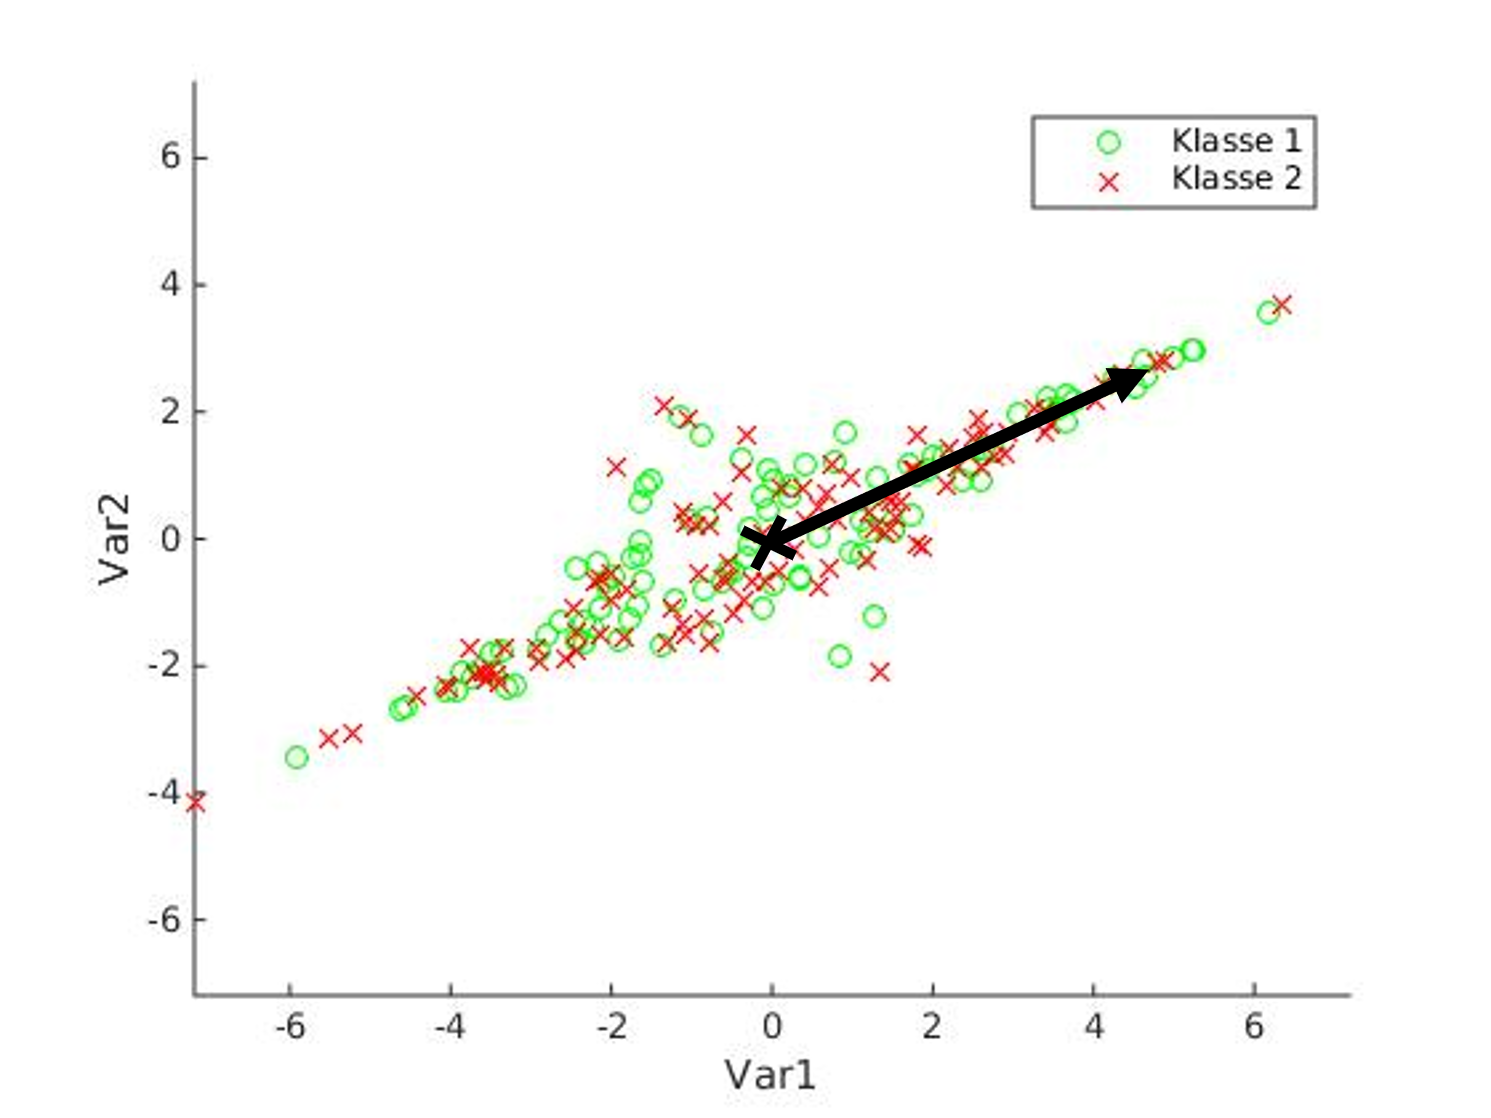
\includegraphics[width=7cm]{assignment4_data/plots/A2b_bild1.png}
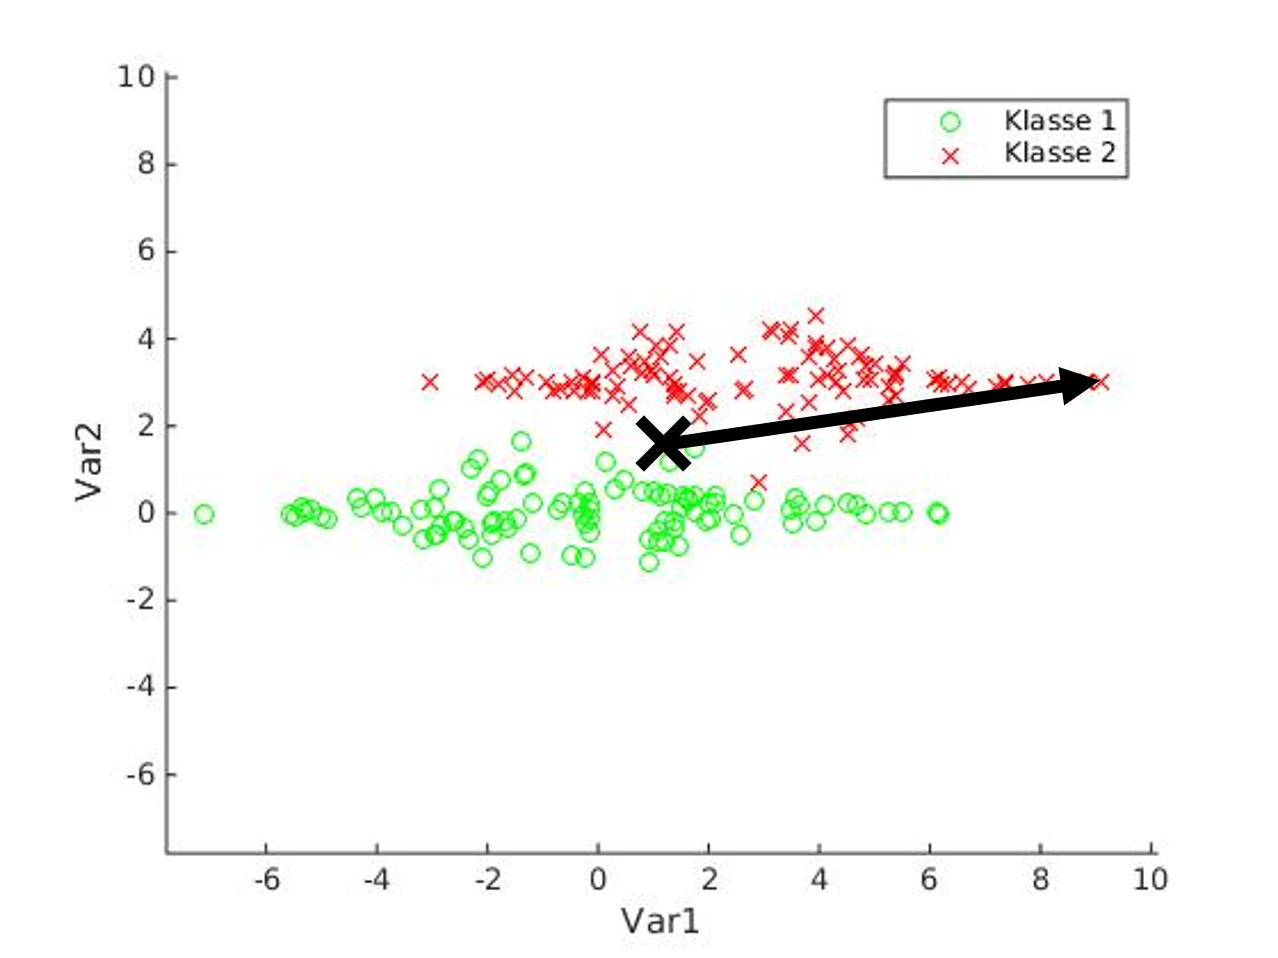
\includegraphics[width=7cm]{assignment4_data/plots/A2b_bild2.png}\\
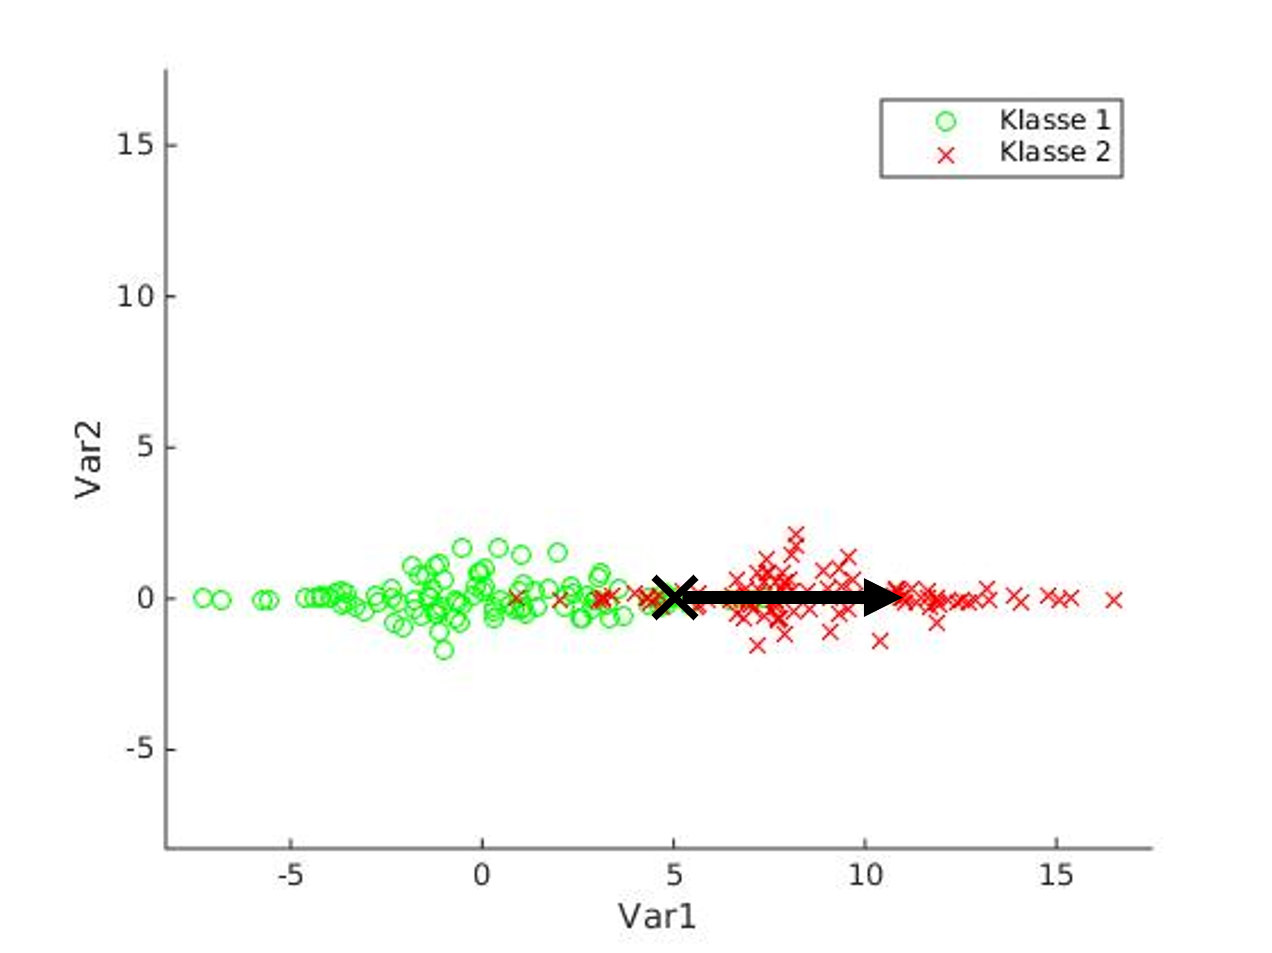
\includegraphics[width=7cm]{assignment4_data/plots/A2b_bild3.png}
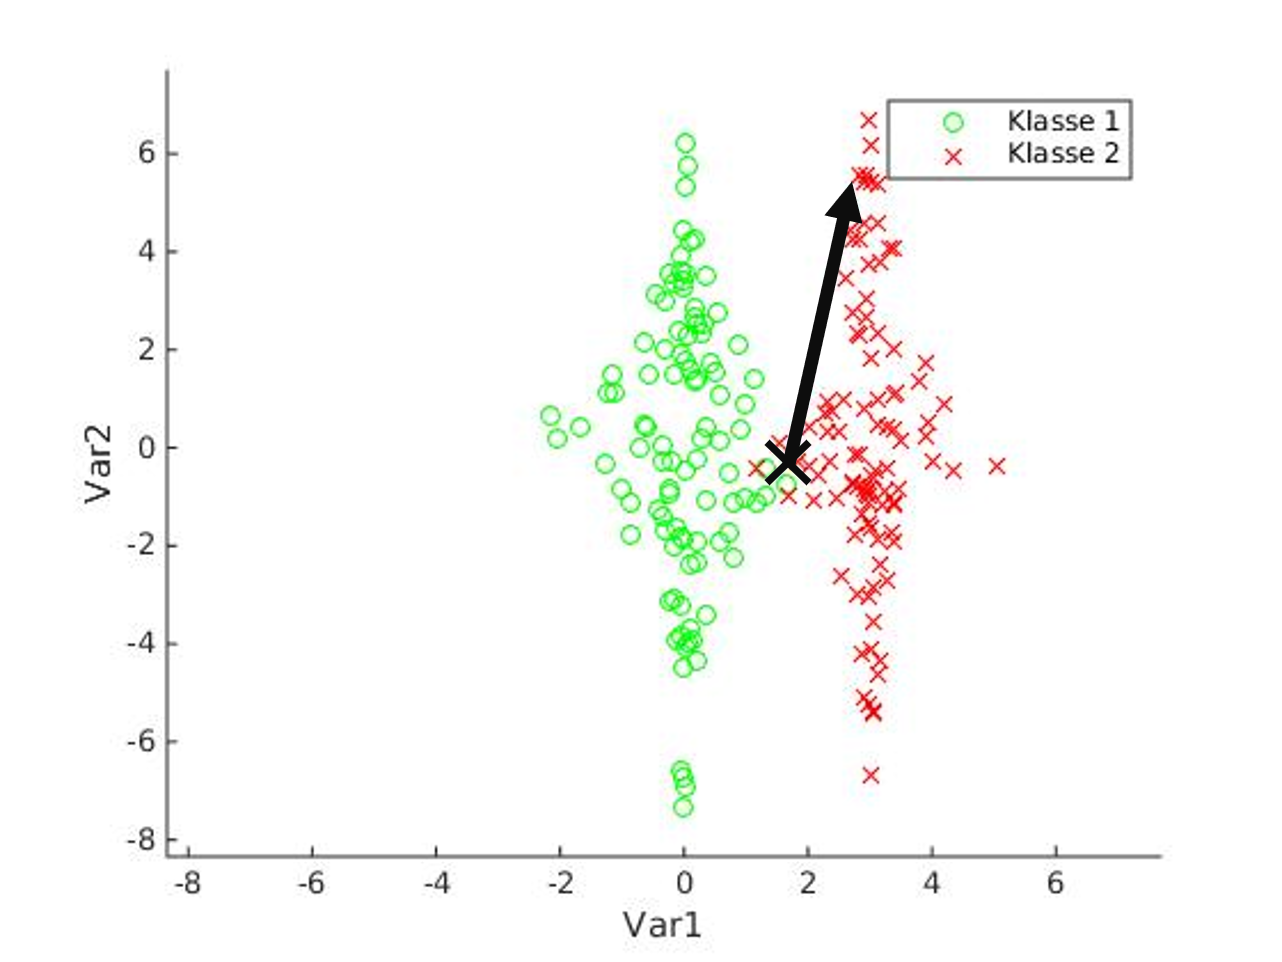
\includegraphics[width=7cm]{assignment4_data/plots/A2b_bild4.png}\\
Für alle Bilder gilt: Der Pfeil stellt die erste Hauptkomponente dar, das Kreuz den Mittelwert.\\
\begin{enumerate}
	\item[a)] Plot 1: Eine Hauptkomponentenanalyse bietet sich hier an. Es ist klar, dass die Daten in die Richtung der ersten Hauptkomponente sehr viel mehr gestreut sind als in die Richtung vertikal dazu. Das bedeutet, dass man einen Großteil der Information, die in den Daten steckt, schon erhält, wenn man sich nur diese eine Richtung anschaut.\\
	Plot 2: Hier ist eine Hauptkomponentenanalyse zwar möglich, allerdings gehen relativ viele Daten verloren, weil die Daten in eine Richtung zwar mehr streuen als in die andere, aber auch in die andere Richtung die Varianz noch relativ hoch ist.\\
	Plot 3: Hier bietet sich die Hauptkomponentenanalyse besonders an, weil die Daten fast nur in eine Richtung streuen.\\
	Plot 4: Hier streuen die Daten in eine Richtung fast genauso wie in die dazu vertikale, eine Hauptkomponentenanalyse bietet sich also nicht an.
	\item[b)] Plot 1: Die entstehende Repräsentation der Daten ist für die Klassifikation nutzlos, weil beide Klassen an jeder Stelle etwa gleich stark vertreten sind.\\
	Plot 2: Die entstehen Repräsentation ist nicht besonders nützlich. Man kann zwar wahrscheinlich einige Datenpunkte richtig klassifizieren, aber eine Trennung der Daten nach Var2 wäre sehr viel einfacher und aussagekräftiger.\\
	Plot 3: Die entstehende Repräsentation ist für die Klassifikation sehr gut geeignet, da lediglich ein Schwellenwert gewählt werden muss, der zwischen den beiden Klassen unterscheidet.\\
	Plot 4: Siehe Plot 1.
\end{enumerate}
\subsection*{c)}
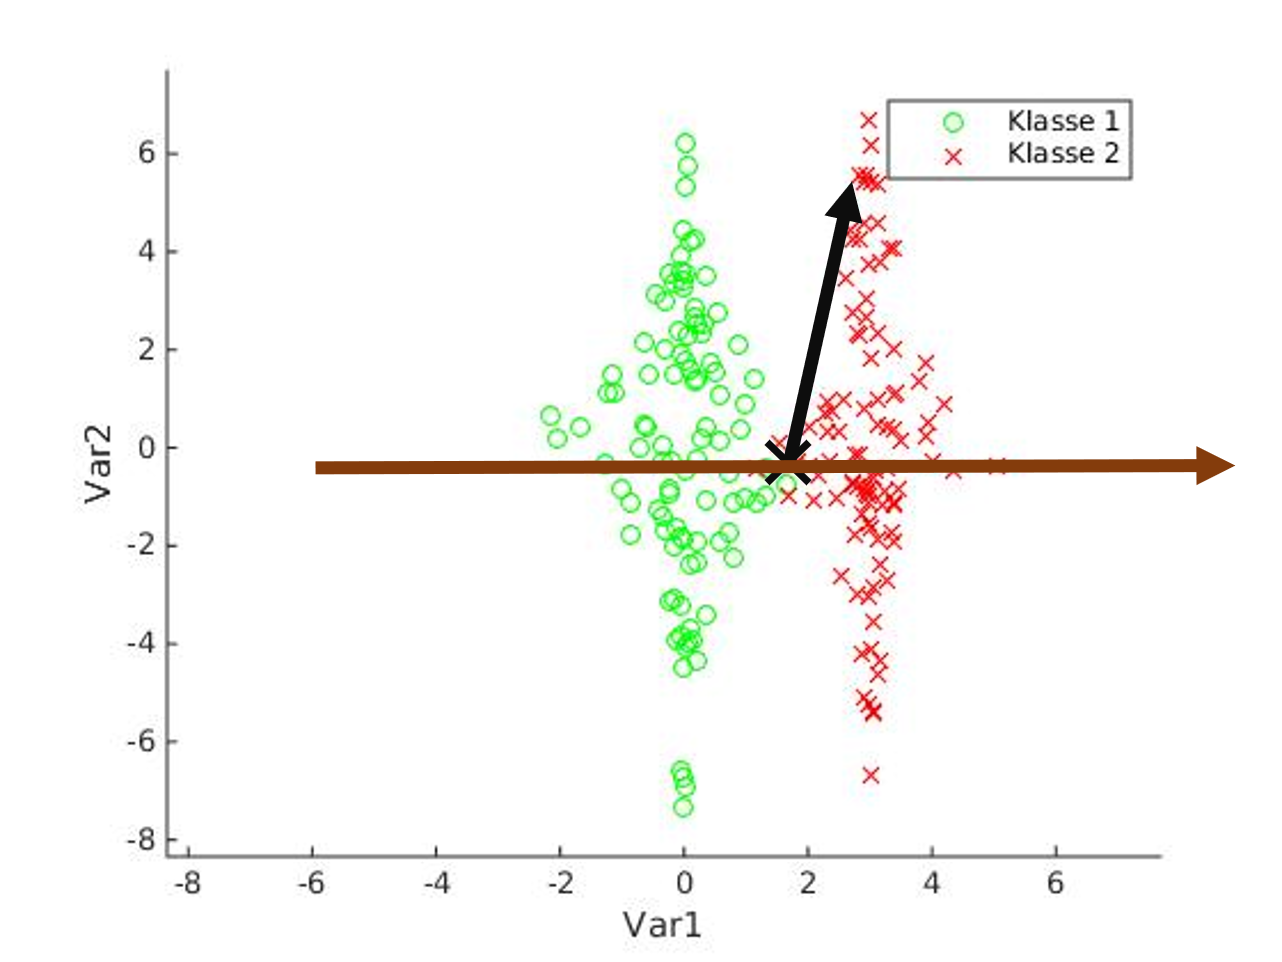
\includegraphics[width=10cm]{assignment4_data/plots/A2c_bild4.png}\\
Der braune Pfeil ist der Unterraum auf den die LDA die Daten projeziert.\\
Bei der PCA wird der neue Unterraum einfach nur hinsichtlich der maximalen Varianz ausgewählt. Der neue Hauptkomponent zeigt einfach in die Richtung mit der höchsten Varianz. Wenn die Daten innerhalb einer Klasse mehr streuen als zwischen den Klassen macht das wenig Sinn.\\
Bei der LDA dagegen geht es um das Verhältnis der Mittelpunkte zur Streuung innerhalb einer Klasse. Dabei soll der Abstand der Mittelpunkte im neuen Unterraum möglichst groß, die Streuung dagegen minimal sein. In dem Fall des Plots 4 bedeutet dies, dass einfach auf einen waagerechten Vektor projeziert wird.\\
Das ist für die Klassifikation sinnvoll, weil dadurch die beiden Klassen so gut möglich getrennt werden. Allerdings geht auch eine Menge Information verloren, nämlich die Varianz der Klassen in Var2. Diese würde mit der PCA besser erhalten bleiben. Beide Methoden haben also unterschiedliche Vor- und Nachteile und dementsprechend unterschiedliche Anwendungsgebiete.

\section*{Aufgabe 3:}
\subsection*{(e)}
\begin{center}
	\includegraphics*[scale = 0.75]{assignment4_data/plots/q3_e.png}
\end{center}

\subsection*{(f)}
Zum einen ist es sinnvoll auf diese Daten PCA anzuwenden, da die ersten beiden Merkmale eine Streuung von ueber 97\% haben und somit die anderen beiden relativ unwichtig erscheinen. Mit dieser Dimensionsreduktion kann man auch deutlich Setosa von den anderen beiden unterscheiden und sehr sicher klassifizieren.\\
Zum anderen hingegen sind Werte von Versicolor und Virginica ziemlich nahe beieinander und somit nicht so einfach unterscheidbar, wenn man nicht weiß welche Art die Lillien haben. 
\end{document}